% \date{May 14, 2024}
% \author{Deralive}
% \title{华东师范大学软件学院实验报告模板}
% 注意事项:编译两次,以确保目录、页码完整显示

\def\allfiles{}

%————————————多文件编译————————————%
% \ifx\allfiles\undefined
% 	    \begin{document}
% \else
% \fi

% Content

% \ifx\allfiles\undefined
% 	    \end{document}
% 	\else
% 	\fi
%—————————————————————————————————%

\documentclass[14pt,a4paper,UTF8,twoside]{article}

\usepackage{amsmath}
\usepackage{graphicx}
\usepackage{geometry} 
\usepackage{ctex}
\usepackage{multicol}
\usepackage{booktabs} % 表格库
\usepackage{titlesec} % 标题库
\usepackage{fancyhdr} % 页眉页脚库
\usepackage{lastpage} % 页码数库
\usepackage{listings} % 代码块包
\usepackage{xcolor}
\usepackage[hidelinks]{hyperref}
\usepackage{tikz}
\usepackage{tikz-qtree}
\usepackage{fontspec} % 允许设置字体
\usepackage{unicode-math} % 允许数学公式使用特定字体
\usepackage{mwe}
\usepackage{zhlipsum} % 中文乱数文本
\usepackage{amsmath}
\usepackage{xcolor}
\usepackage{float} % 浮动体环境
\usepackage{subcaption} % 子图包
\usepackage{biblatex}
\usepackage{array}
\usepackage{multirow}
\addbibresource{references.bib} % 指定你的.bib文件名称

\definecolor{mygreen}{rgb}{0,0.6,0}
\definecolor{mygray}{rgb}{0.5,0.5,0.5}
\definecolor{mymauve}{rgb}{0.58,0,0.82}

\date{} % 留空,以让编译时去除日期

%———————————————注意事项—————————————————%

% 1、如果编译显示失败,但没有错误信息,就是 filename.pdf 正在被占用
% 2、在文件夹中的终端使用 Windows > xelatex filename.tex 也可编译

%—————————————华东师范大学———————————————%

% 论文制作时须加页眉,页眉从中文摘要开始至论文末
% 偶数页码内容为:华东师范大学硕士学位论文,奇数页码内容为学位论文题目

%————————定义 \section 的标题样式————————%

% 注意:\chapter 等命令,内部使用的是 \thispagestyle{plain} 的排版格式
% 若需要自己加上页眉,实际是在用 \thispagestyle{fancy} 的排版格式
% 加上下面这一段指令,就能够让 \section 也使用 fancy 的排版格式
% 本质就是让目录、第一页也能够显示页眉、页脚

\fancypagestyle{plain}{
  \pagestyle{fancy}
}

\title{华东师范大学软件学院课程作业} % 模板
\titleformat{\section}
    {\normalfont\bfseries\Large} % 字体大小、字体系列(\bfseries 为加粗)
    {\thesection}{1em}{}

% 设置章节的中文格式
\renewcommand\thesection{\chinese{section} \hspace{0pt}}
\renewcommand\thesubsection{\arabic{subsection} \hspace{0pt}}
% \renewcommand\thesubsubsection{\alph{subsubsection} \hspace{0pt}} % 字母编号
% \hspace{0pt} 是为了确保在章节编号和章节题目之间不要有空格,使得排版更为美观
    
%—————————————页面基础设置———————————————%

\geometry{left=10mm, right=10mm, top=20mm, bottom=20mm}

%————————————设置页眉、页脚——————————————%

\pagestyle{fancy} % 设置 plain style 的属性

% 设置页眉

\fancyhead[RE]{\leftmark} % Right Even 偶数页右侧显示章名 \leftmark 最高级别章名
\fancyhead[LO]{\rightmark} % Left Odd 奇数页左侧显示节名 \rightmark 第二级别节名
\fancyhead[C]{华东师范大学软件学院课程作业} % Center 居中显示
\fancyhead[LE,RO]{~\thepage~} % 在偶数页的左侧,奇数页的右侧显示页码
\renewcommand{\headrulewidth}{1.2pt} % 页眉与正文之间的水平线粗细

% 设置页脚:在每页的右下脚以斜体显示书名

\fancyfoot[RO,RE]{\it Lab Report By \LaTeX} % 使用意大利斜体显示
\renewcommand{\footrulewidth}{0.5pt} % 页脚水平线宽度

% 设置页码:在底部居中显示页码

\pagestyle{fancy}
\fancyfoot[C]{\kaishu 第 \thepage 页 \ 共 \pageref{LastPage} 页} % LastPage 需要二次编译以获取总页数

%——————————————代码块设置———————————————%

\lstset {
    backgroundcolor=\color{white},   % choose the background color; you must add \usepackage{color} or \usepackage{xcolor}
    basicstyle=\footnotesize,        % the size of the fonts that are used for the code
    breakatwhitespace=false,         % sets if automatic breaks should only happen at whitespace
    breaklines=true,                 % sets automatic line breaking
    captionpos=bl,                   % sets the caption-position to bottom
    commentstyle=\color{mygreen},    % comment style
    deletekeywords={...},            % if you want to delete keywords from the given language
    escapeinside={\%*}{*},           % if you want to add LaTeX within your code
    extendedchars=true,              % lets you use non-ASCII characters; for 8-bits encodings only, does not work with UTF-8
    frame=single,                    % adds a frame around the code
    keepspaces=true,                 % keeps spaces in text, useful for keeping indentation of code (possibly needs columns=flexible)
    keywordstyle=\color{blue},       % keyword style
    % language=Python,               % the language of the code
    morekeywords={*,...},            % if you want to add more keywords to the set
    numbers=left,                    % where to put the line-numbers; possible values are (none, left, right)
    numbersep=5pt,                   % how far the line-numbers are from the code
    numberstyle=\tiny\color{mygray}, % the style that is used for the line-numbers
    rulecolor=\color{black},         % if not set, the frame-color may be changed on line-breaks within not-black text (e.g. comments (green here))
    showspaces=false,                % show spaces everywhere adding particular underscores; it overrides 'showstringspaces'
    showstringspaces=false,          % underline spaces within strings only
    showtabs=false,                  % show tabs within strings adding particular underscores
    stepnumber=1,                    % the step between two line-numbers. If it's 1, each line will be numbered
    stringstyle=\color{orange},      % string literal style
    tabsize=2,                       % sets default tabsize to 2 spaces
    % title=Python Code              % show the filename of files included with \lstinputlisting; also try caption instead of title
}

% 注释掉的部分用于后续插入代码,参数可调整,格式如下:

% 1、直接插入
% \begin{lstlisting}[language = ? , title = { ? } ]
%       Your code here.
% \end{lstlisting}

% 2、文件插入
% \lstinputlisting[language = C , title = ?.c] {filename.c}

%———————————————字体设置————————————————%

% \setCJKmainfont{SimSun} % 设置正文罗马族的 CJK 字体
% \renewcommand{\normalsize}{\fontsize{12pt}{15pt}\selectfont} % 设置正文字号
\linespread{1.2}

%——————————————————————————————————————%

%———————————————超链接设置——————————————%

\hypersetup{
    pdfstartview=FitH, % 设置PDF文档打开时的初始视图为页面宽度适应窗口宽度(即页面水平适应)
    CJKbookmarks=true, % 用对CJK(中文、日文、韩文)字符的书签支持,确保这些字符在书签中正确显示
    bookmarksnumbered=true, % 书签带有章节编号。这对有章节编号的文档很有用
    bookmarksopen=true, % 文档打开时,书签树是展开的,方便查看所有书签
    colorlinks, % 启用彩色链接。这样,链接在PDF中会显示为彩色,而不是默认的方框
    pdfborder=001, % 设置PDF文档中链接的边框样式。001 表示链接周围没有边框,仅在单击时显示一个矩形
    linkcolor=blue, % 设置文档内部链接(如目录中的章节链接)的颜色为蓝色
    anchorcolor=blue, % 设置锚点链接(即目标在同一文档内的链接)的颜色为蓝色
    citecolor=blue, % 设置引用(如文献引用)的颜色为蓝色
}

%——————————————导言区结束,进入正文部分———————————————%

%——————————————————————————————————————%

\begin{document}

\maketitle

\begin{center} % \extracolsep{\fill} 拉伸到页面最大宽度前,保证居中显示

  \begin{tabular*}{\textwidth}{@{\extracolsep{\fill}} l  l  l }
    \hline
    课程名称:软件质量分析 &  年级:2023级本科  &  姓名:张梓卫 \\
    作业主题:总结软件可靠性定义 & 学号:10235101526 & 作业日期:2024/10/10 \\
    指导老师:陈仪香 & 组号: \\
    \hline
  \end{tabular*}

\end{center}

\tableofcontents % 目录也需要二次编译

\section{系统级软件FMEA的定义}

\subsection{定义}
系统级软件FMEA(Failure Modes and Effects Analysis)通过识别软件失效模式*,分析造成的后果,研究分析各种失效模式产生的原因,
寻找消除和减少其有害后果的方法,以尽早发现潜在的问题,并采取相应的措施,从而提高软件的可靠性和安全性。
用于预防软件系统中的潜在问题,确保系统的可靠性和安全性。常用于嵌入式领域。

FMEA的目标是识别可能的故障源头,评估这些故障的影响,并在故障实际发生前采取预防或减轻措施。
FMEA通常应用于软件开发的早期阶段,以便在设计阶段就能发现潜在的问题。

*\textbf{软件失效模式}:软件失效(软件故障引起的,泛指程序运行中丧失全部或部分功能)发生的不同方式。分析它是软件FMEA的基础。

\section{FMEA的步骤}

\subsection{系统定义以确定分析级别和分析对象}

功能:确定分析重点,说明系统主要和次要功能,

优势:根据软件系统的功能、结构特征等确定系统的分析级别,在高层较易全面分析,在低层的分析更深入。

注意:若无法全面分析,可在分析前确定分析重点,识别对系统功能和安全性影响较大的危险事件作为FMEA分析的重点。

\subsection{确定分析分析对象的失效模式}

功能:针对每个分析对象,参考失效模式。

举例:响应超时、输出错误。

\subsection{分析失效模式的可能原因}

功能:尽可能全面分析失效原因,为制定改进措施提供依据。

一般失效原因种,可以分为多种具体失效原因。

归类如下:

\begin{multicols}{2}
\begin{itemize}
    \item 逻辑遗漏或执行错误
    \begin{itemize}
        \item 遗忘细节或步骤
        \item 逻辑重复
        \item 忽略极限条件
        \item 不必要的函数
        \item 需求的错误表达
        \item 未进行条件测试
        \item 检查错误变量
        \item 循环错误
    \end{itemize}
    \item 算法的编码错误
    \begin{itemize}
        \item 等式不完整或不正确
        \item 丢失运算结果
        \item 操作数错误
        \item 括号使用错误
        \item 精度损失
        \item 含入和舍去错误
        \item 混合类型
        \item 标记习惯不正确
    \end{itemize}
    \item 软硬件接口失效
    \begin{itemize}
        \item 中断句柄错误
        \item I/O时序错误
        \item 时序错误导致数据丢失
        \item 子函数调用不当
        \item 子函数调用位置错误
        \item 调用不存在的子函数
        \item 子函数不一致
    \end{itemize}
    \item 数据错误或丢失
    \begin{itemize}
        \item 传感器数据错误或丢失
        \item 操作数据错误或丢失
        \item 嵌入到表中的数据错误或丢失
        \item 外部数据错误或丢失
        \item 输出数据错误或丢失
        \item 输入数据错误或丢失
    \end{itemize}
    \item 数据操作错误
    \begin{itemize}
        \item 数据初始化错误
        \item 数据存取错误
        \item 数据打包解包错误
        \item 标志或索引设置不当
        \item 变量参考错误数据
        \item 数据越界
        \item 变量缩放比率或单位不正确
        \item 变量维度不正确
        \item 变量类型错误
        \item 变量下标错误
        \item 数据范围不对
    \end{itemize}
\end{itemize}
\end{multicols}

\subsection{分析失效影响及其严重性}

功能:分析每个失效模式对局部、高一层,直至整个系统的影响,以及
失效影响的严重性,以识别软件失效所造成后果的严重程度,以便按照优先级为不同的情况制定改进措施。

\subsection{制定改进措施}

功能:根据上述分析得到的失效原因和影响的严重性,确定需要采取的改进措施。

\textbf{改进方式}:

\subsubsection{软件层面}

修改软件需求、设计或编码
中的缺陷,增加软件的防护措施。

\subsubsection{硬件层面}

增加硬件防护措施。

\subsubsection{FMEA表格}

进行软件FMEA时, 应填写FMEA表。该表应能完整地体现分析的目的和取得成果。

\noindent
\begin{minipage}{\textwidth}
    \centering
    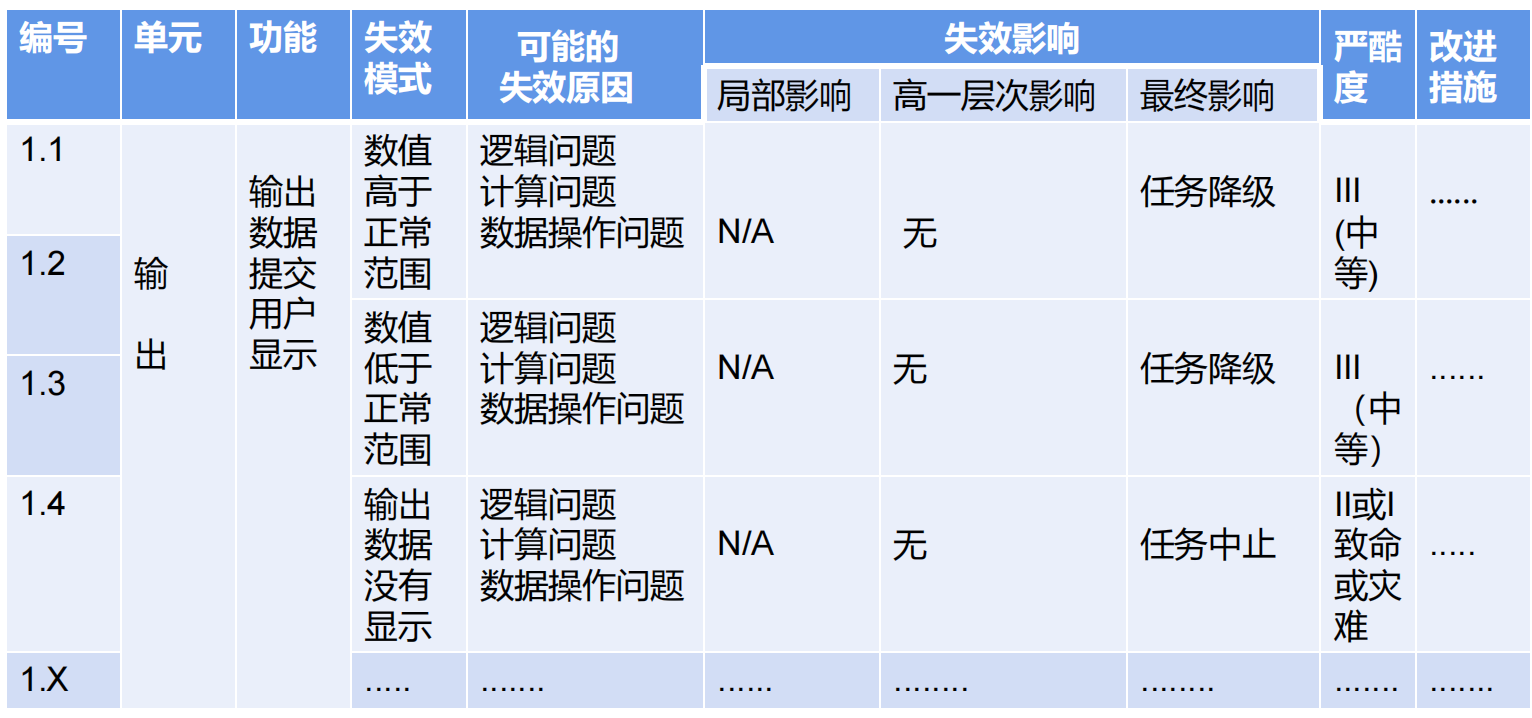
\includegraphics[width=0.6\textwidth]{img3/table.png}
    % \caption{figure}{FMEA表格}
    \label{fig:FMEA}
\end{minipage}

\section{选做题作业}
\section*{构建 Jelinski-Moranda 模型}

\subsection*{收集并处理数据}

首先,处理给定的失效时间数据:

\begin{lstlisting} [language=Python]
# 给定的失效时间数据(单位时间)
failure_times = [15, 13, 9, 10, 21, 23, 18, 22, 17, 16]

# 计算累计失效时间和总测试时间
cumulative_times = []
total_time = 0
for t in failure_times:
    total_time += t
    cumulative_times.append(total_time)

S = total_time          # 总的测试时间
n = len(failure_times)  # 已发生的失效次数
\end{lstlisting}

\subsection*{估计参数 \( N \)(初始故障总数)}

Jelinski-Moranda 模型的关键是估计软件中的初始故障总数 \( N \)。需要解以下方程:

\[
\sum_{k=1}^{n} \frac{1}{N - (k - 1)} = \frac{n}{S}
\]

由于无法直接求解,我们使用数值方法(如二分法)来估计 \( N \):

\begin{lstlisting} [language=Python]
def equation(N, n, S):
    left_sum = sum([1 / (N - (k - 1)) for k in range(1, n + 1)])
    right_sum = n / S
    return left_sum - right_sum

from scipy.optimize import root_scalar

def func(N):
    return equation(N, n, S)

# 设置求解区间,N > n
sol = root_scalar(func, bracket=[n + 1, n + 1000], method='bisect')
N_estimated = sol.root
print(f"估计的 N 值为: {N_estimated}")
\end{lstlisting}

\subsection*{估计参数 \( \phi \)}

计算参数 \( \phi \):

\[
\phi = \frac{n}{\sum\limits_{k=1}^{n} (N - k + 1) \cdot T_k}
\]

其中,\( T_k \) 为第 \( k \) 次失效的间隔时间。

\begin{lstlisting} [language=Python]
# 计算分母
denominator = sum([(N_estimated - k + 1) * failure_times[k - 1] for k in range(1, n + 1)])

# 计算 φ
phi = n / denominator
print(f"估计的 φ 值为: {phi}")
\end{lstlisting}

\subsection*{计算第 11 次失效前的失效率 \( \lambda \)}

\[
\lambda_{n+1} = \phi \cdot (N - n)
\]

\begin{lstlisting} [language=Python]
lambda_11 = phi * (N_estimated - n)
print(f"第 11 次失效前的失效率 λ 为: {lambda_11}")
\end{lstlisting}

\subsection*{计算平均失效前时间(MTTF)}

\[
\text{MTTF} = \frac{1}{\lambda_{n+1}}
\]

\begin{lstlisting} [language=Python]
MTTF = 1 / lambda_11
print(f"平均失效前时间(MTTF)为: {MTTF}")
\end{lstlisting}

\subsection*{计算在 MTTF 时的软件可靠度 \( R(t) \)}

\[
R(t) = e^{-\lambda_{n+1} \cdot t}
\]

令 \( t = \text{MTTF} \),则:

\begin{lstlisting} [language=Python]
import math

t = MTTF
R_t = math.exp(-lambda_11 * t)
print(f"在时间 t = MTTF 时的软件可靠度 R(t) 为: {R_t}")
\end{lstlisting}

\subsection*{计算不可靠度 \( U(t) \)}

\[
U(t) = 1 - R(t)
\]

\begin{lstlisting} [language=Python]
U_t = 1 - R_t
print(f"在时间 t = MTTF 时的软件不可靠度 U(t) 为: {U_t}")
\end{lstlisting}

\subsection*{计算失效密度 \( f(t) \)}

\[
f(t) = \lambda_{n+1} \cdot e^{-\lambda_{n+1} \cdot t}
\]

\begin{lstlisting} [language=Python]
f_t = lambda_11 * math.exp(-lambda_11 * t)
print(f"在时间 t = MTTF 时的失效密度 f(t) 为: {f_t}")
\end{lstlisting}

\subsection*{完整代码}

\begin{lstlisting} [language=Python]
failure_times = [15, 13, 9, 10, 21, 23, 18, 22, 17, 16]
cumulative_times = []
total_time = 0
for t in failure_times:
    total_time += t
    cumulative_times.append(total_time)

S = total_time
n = len(failure_times)

def equation(N, n, S):
    left_sum = sum([1 / (N - (k - 1)) for k in range(1, n + 1)])
    right_sum = n / S
    return left_sum - right_sum

from scipy.optimize import root_scalar

def func(N):
    return equation(N, n, S)

sol = root_scalar(func, bracket=[n + 1, n + 1000], method='bisect')
N_estimated = sol.root
print(f"估计的 N 值为: {N_estimated}")

denominator = sum([(N_estimated - k + 1) * failure_times[k - 1] for k in range(1, n + 1)])
phi = n / denominator
print(f"估计的 φ 值为: {phi}")

lambda_11 = phi * (N_estimated - n)
print(f"第 11 次失效前的失效率 λ 为: {lambda_11}")

MTTF = 1 / lambda_11
print(f"平均失效前时间(MTTF)为: {MTTF}")

import math
t = MTTF
R_t = math.exp(-lambda_11 * t)
print(f"在时间 t = MTTF 时的软件可靠度 R(t) 为: {R_t}")

U_t = 1 - R_t
print(f"在时间 t = MTTF 时的软件不可靠度 U(t) 为: {U_t}")

f_t = lambda_11 * math.exp(-lambda_11 * t)
print(f"在时间 t = MTTF 时的失效密度 f(t) 为: {f_t}")
\end{lstlisting}

\subsection*{运行结果}

\begin{verbatim}
估计的 N 值为: 169.00000000000006
估计的 φ 值为: 0.0003717857830703583
第 11 次失效前的失效率 λ 为: 0.05918594751117227
平均失效前时间(MTTF)为: 16.889800000000006
在时间 t = MTTF 时的软件可靠度 R(t) 为: 0.3678794411714422
在时间 t = MTTF 时的软件不可靠度 U(t) 为: 0.6321205588285578
在时间 t = MTTF 时的失效密度 f(t) 为: 0.02186010370865581
\end{verbatim}

\subsection*{结论}

\begin{itemize}
    \item \textbf{软件可靠度 \( R(t) \)}:在第 11 次失效发生的平均时间(MTTF)时,软件可靠度约为 \textbf{0.3679}。
    \item \textbf{不可靠度 \( U(t) \)}:在同一时间点,软件不可靠度约为 \textbf{0.6321}。
    \item \textbf{失效密度 \( f(t) \)}:在 MTTF 时的失效密度约为 \textbf{0.02186}。
    \item \textbf{平均失效前时间(MTTF)}:约为 \textbf{16.89} 时间单位。
\end{itemize}

\section{其余笔记}

\subsection{系统级软件FMEA}

在软件开发阶段的早期,用于发现软件需求或软件体系结构等存在的缺陷。主要分析对象:\textbf{软件需求分析阶段的软件功能或设计阶段的软件部件}

失效模式(9种):

\begin{itemize}
  \item (1) 操作系统挂起
  \item (2) 程序挂起
  \item (3)程序失败:程序不能启动;程序运行不能终止;程序不能退出
  \item (4)输入问题:错误输入被接受;正确输入被拒绝;描述不正确或遗漏;参数不正确或遗漏
  \item (5)输出问题: 错误的格式;不正确的结果或数据;不完全或遗漏;拼写问题、语法问题
  \item (6)未达到要求的性能:错误的格式;不正确的结果或数据;不完全或遗漏;拼写问题、语法问题
  \item (7)发现整个产品失败
  \item (8)系统错误信
  \item (9)其他:程序运行改变了系统配置参数;程序运行改变了其他程序的运行结果数据
\end{itemize}

软件失效模式分为两类:通用失效模式和详细失效模式。

详细失效模式是对通用失效模式的细化,又分为五子类:输入失效、输出失效、程序失效、未满足功能及性能要求失效、其他类型。

\section*{软件失效模式示例}

\begin{multicols}{2}
\begin{itemize}
    \item \textbf{软件通用失效模式}
    \begin{itemize}
        \item 运行时不符合要求
        \item 输入不符合要求
        \item 输出不符合要求
    \end{itemize}

    \item \textbf{软件详细失效模式}
    \begin{itemize}
        \item 输入失效
        \begin{itemize}
            \item 未收到输入
            \item 收到错误输入
            \item 收到数据轻微超差
            \item 收到数据中度超差
            \item 收到数据严重超差
            \item 收到参数不完全或遗漏
            \item 其他
        \end{itemize}

        \item 输出失效
        \begin{itemize}
            \item 输出结果错误(如输出项缺损或多余等)
            \item 输出数据精度轻微超差
            \item 输出数据精度中度超差
            \item 输出数据精度严重超差
            \item 输出参数不完全或遗漏
            \item 输出格式错误
            \item 输出打印字符不符合要求
            \item 输出拼写/语法错误
            \item 其他
        \end{itemize}

        \item 程序失效
        \begin{itemize}
            \item 程序无法启动
            \item 程序运行中断
            \item 程序无法终止
            \item 程序无法退出
            \item 程序陷入死循环
            \item 程序运行影响其他单元或环境
            \item 程序轻微超时
            \item 程序明显超时
            \item 程序严重超时
            \item 其他
        \end{itemize}

        \item 其他失效
        \begin{itemize}
            \item 程序改变配置无法启动
            \item 程序改变其他程序数据
            \item 操作系统错误
            \item 硬件错误
            \item 整个系统错误
            \item 人为操作错误
            \item 接口失效
            \item I/O定时不准致数据丢失
            \item 维护不合理
            \item 其他
        \end{itemize}
    \end{itemize}
\end{itemize}
\end{multicols}

\section{实施注意事项}

\subsection{基础内容}

1.软件FMEA的应用重点在软件开发过程的早期,找出可能存在的与功能和性能相关的缺陷,以尽早完善需求分析与概要设计。
2.根据分析阶段和级别不同分为系统级和详细级。

\subsection{主要内容}

1. 软件失效模式是软件FMEA的基础。失效模式的分析是否全面
合理决定了软件FMEA的分析效果,是整个分析过程中最为关键的
一步。

2.软件失效原因是由于软件缺陷在运行时被触发而产生的。对软件
FMEA失效原因分析就是要找出潜在的软件缺陷。

3. 失效影响既可对每一个软件失效模式造成的“局部、高一层次和最
终”三级影响进行分析,又可对“具备、高一层次”的影响进行分析,或直
接对“局部、最终”影响进行分析。

4.分析对象既可以是软件功能模块、软件部件,又可以是底层的软件单元

\section{参考文献}

\begin{itemize}
    \item \href{https://arxiv.org/pdf/1108.5185}{\underline{https://arxiv.org/pdf/1108.5185}}
    \item J-M 模型的计算机实现:\href{https://www.wdfxw.net/doc20562618.htm}{\underline[https://www.wdfxw.net/doc20562618.htm]}
\end{itemize}

\end{document}